\newpage
\section{Numérisation}
Beaucoup de phénomènes physiques sont continus (analogues) et nécessitent d'être numérisés afin de pouvoir être manipulés par ordinateur. Cette numérisation demande l'échantillonnage et la quantification du phénomène analogue.

\subsection{Échantillonnage}
Dans la vraie vie, il est impossible de pouvoir enregistrer les données d'une expérience à chaque instant. Autrement, il faudrait une quantité infinie de mémoire et, par la suite, faire l'analyse de cette quantité astronomique de données serait un enfer. Alors, on prend des mesures à intervalles réguliers, ce qu'on nomme l'échantillonage. 

\begin{figure}[H]
    \centering
        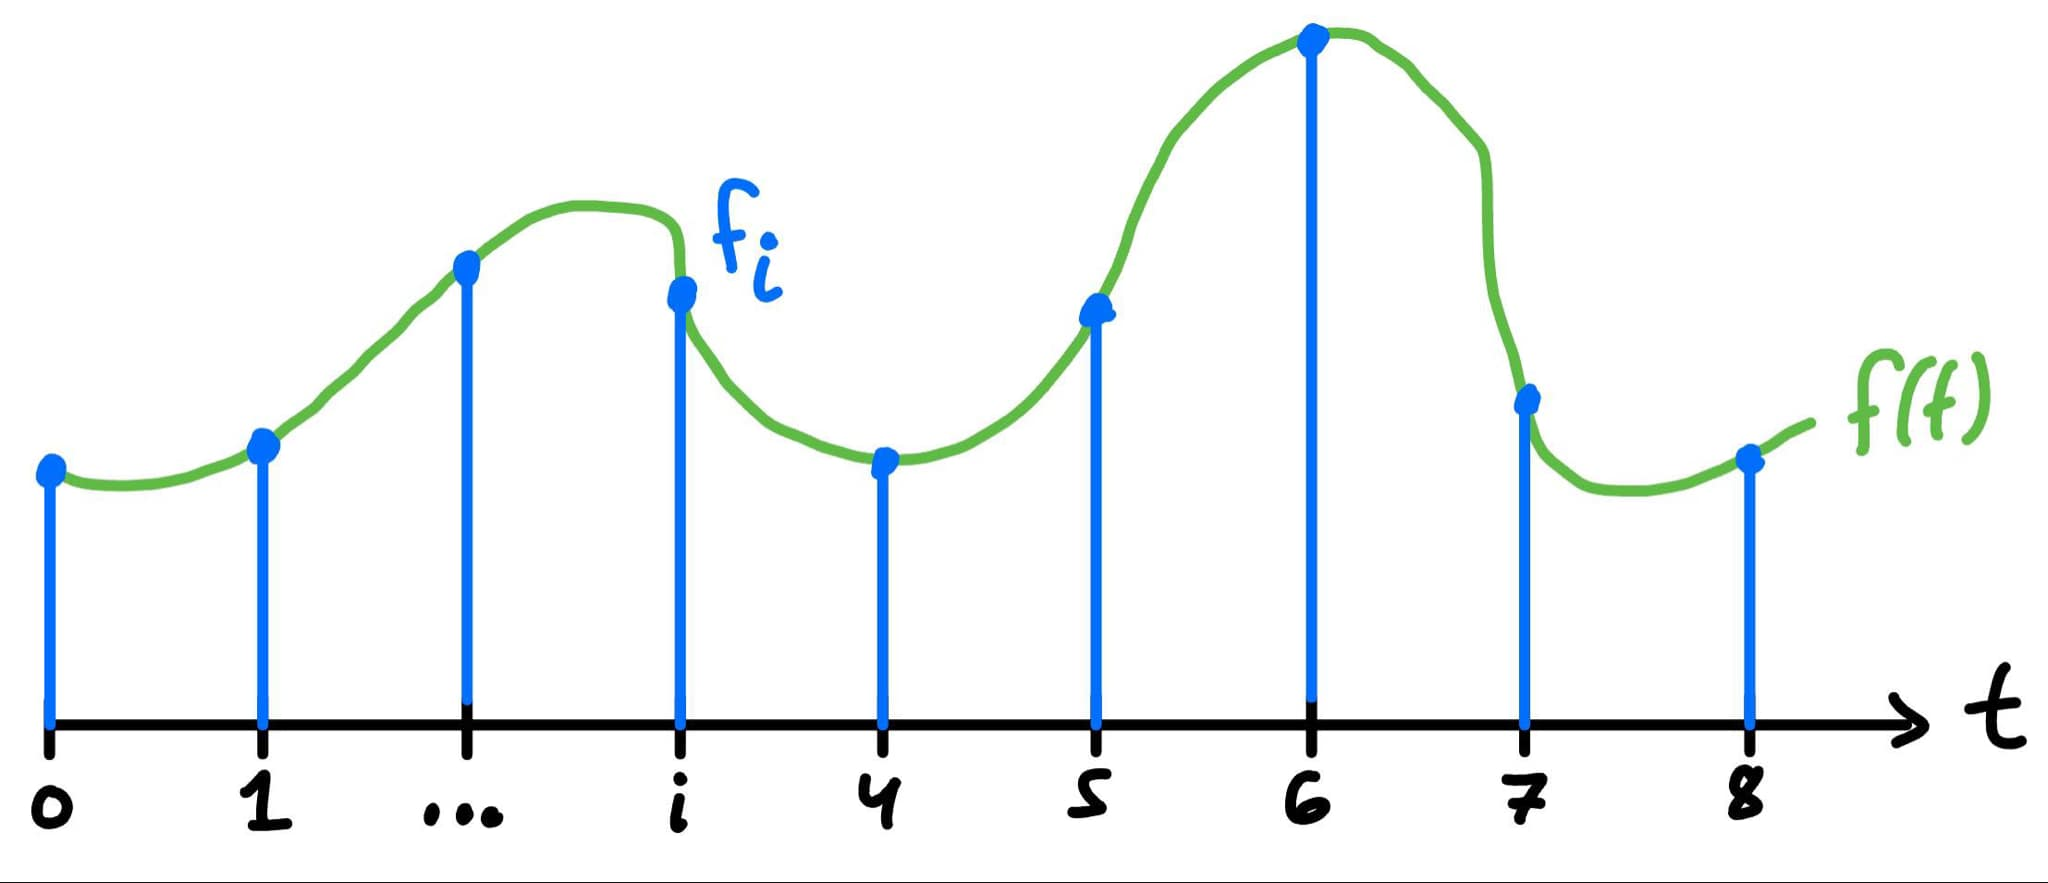
\includegraphics[width=0.5\textwidth]{images/ch6/echantillonnage.jpg}
        \caption{Échantillonnage (en bleu) d'une fonction $f(t)$}
    \end{figure}

Le rythme auquel on décide de prendre les mesures se nomme la fréquence d'échantillonage $f_s$. Évidemment, plus la fréquence d'échantillonage est grande, plus nos mesures "ont l'air" du phénomène analogue qu'elles décrivent. Cependant, une trop grande fréquence d'échantillonage donne beaucoup de données et, dans ce cas, peut-être que les mesures seront redondantes ou bien que leur traitement sera lent vu leur quantité. Par ailleurs, une trop petite fréquence d'échantillonage n'est peut-être pas suffisante pour représenter fidèlement le phénomène qu'on mesure. Ainsi, pour avoir le maximum d'informations avec le moins de données, quelle fréquence d'échantillonage faut-il choisir?


